%%%%%%%%%%%%%%%%%%%%%%%%%%%%%%%%%%%%%%%%%%%%%%%%%%%%%%%%%%%%
\subsubsection*{Introduction}
Neutrinos, unlike the other fermions of the Standard Model of particle physics, could be Majorana particles, that is, indistinguishable from their antiparticles. The existence of Majorana neutrinos would have profound implications in particle physics and cosmology. 

 If neutrinos are Majorana particles, there must exist a new scale of physics (at a level inversely proportional to the neutrino masses) that characterises underlying dynamics beyond the Standard Model. The existence of such a new scale provides the simplest explanation of why neutrino masses are so much lighter than the charged fermions. Indeed,  understanding the new physics that underlies neutrino masses is one of the most important open questions in particle physics, and it could have profound implications in our comprehension of the mechanism of symmetry breaking, the origin of mass and the flavor problem. 

The existence of Majorana neutrinos would imply that lepton number is not conserved, which could be the origin of the matter-antimatter asymmetry observed in the Universe. The new physics related to neutrino masses could provide a new mechanism to generate the asymmetry called leptogenesis. Although the predictions are model dependent, two essential ingredients must be confirmed experimentally: 1) the violation of lepton number and 2) CP violation in the lepton sector. 

The only practical way to establish experimentally that neutrinos are their own antiparticles and that lepton number is not conserved is the detection of neutrinoless double beta decay (\bbonu). This is a hypothetical, very slow nuclear transition in which a nucleus with $Z$ protons decays into a nucleus with $Z+2$ protons and the same mass number $A$, emitting two electrons that carry essentially all the energy released (\Qbb). The process can occur if and only if neutrinos are Majorana particles. 

%%%%%%%%%%%%%%%%%%%%%%%%%%%%%%%%%%%%%%%%%%%%%%%%%%%%%%%%%%%%
\subsubsection*{The experimental landscape}

The detectors used in double beta decay searches are designed to measure the energy of the radiation emitted by a \bb\ source. In the case of \bbonu, the sum of the kinetic energies of the two released electrons is fixed by the mass difference between the parent and the daughter nuclei: $Q_{\bb} \equiv M(Z,A)-M(Z+2,A)$. However, due to the finite energy resolution of any detector, \bbonu\ events are reconstructed within an energy region centered around \Qbb, typically following a gaussian distribution (Region of Interest or ROI). Other processes occurring in the detector can fall in the ROI, becoming a background and compromising drastically the expected sensitivity. It follows that \bbonu\ experiments require {\bf excellent energy resolution}, and indeed the field was traditionally dominated by germanium calorimeters, devices with superb resolution.

All double beta decay experiments have to deal with an intrinsic background, the \bbtnu, the standard process of a double $\beta$-decay with the emission of two neutrinos, that can only be suppressed by means of good energy resolution. Backgrounds of cosmogenic origin force the {\bf underground operation of the detectors}. Natural radioactivity emanating from the detector materials and surroundings can easily overwhelm the signal peak, and hence {\bf careful selection of radiopure materials is also essential}. 
{\bf Additional experimental signatures} that allow the distinction between signal and background are certainly a bonus, and this has been in the last few years an important line of work to increase the sensitivity of \bbonu\ detectors. Several other factors such as {\bf detection efficiency} or the {\bf scalability to large masses} must be also taken into account during the design of a double beta decay experiment.
 
 \subsubsection*{Recent results}
 The status of the field has been reviewed recently by the PI\footnote{St. Andrews lectures}.
 Three new-generation experiments, with fiducial masses in the range of the 100 kg, have recently published the results of their searches for \bbonu\ processes. These are: GERDA, a high resolution calorimeter based in Ge-76 diodes; KamLAND-Zen, a low resolution, high-mass, self-shielding liquid scintillator calorimeter, with xenon dissolved in the scintillator; and EXO-200, a liquid xenon (LXe) TPC. All the experiments published negative results and therefore a limit in the period of \bbonu\ processes, \Tonu. This limit can be translated into a limit in the \emph{effective Majorana mass} of the electron neutrino defined as:
\begin{equation}
\mbb = \Big| \sum_{i} U^{2}_{ei} \ m_{i} \Big| \, ,
\end{equation}
%
where $m_{i}$ are the neutrino mass eigenstates and $U_{ei}$ are elements of the neutrino mixing matrix. \mbb\ is related to the period through the equation:

\begin{equation}
(T^{0\nu}_{1/2})^{-1} = G^{0\nu} \ \big|M^{0\nu}\big|^{2} \ \mbb^{2} \, .
\label{eq:Tonu}
\end{equation}

Here, $G^{0\nu}$ is an exactly-calculable phase-space integral for the emission of two electrons and$M^{0\nu}$ is the nuclear matrix element (NME) of the transition, which has to be evaluated theoretically. The uncertainty in the NME affects the value of \mbb\ which can be obtained from \Tonu.
 
GERDA has a resolution of $\sim$0.2 \% FWHM around the \Qbb\ of \GE. The specific background rate in the ROI is $10^{-2}$ \ckky\ and the total exposure deployed 21.6 kg $\times$ yr. The experiment sets a limit $\Tonu > 2 \times 10^{25}$~yr, which translates  in a range for \mbb\ of $[258-649]$~mili electron volts (meV). The lowest value of \mbb\ corresponds to the IBM2 NME set, while the highest value corresponds to the ISM set.

EXO achieves an energy resolution of 3.6\% FWHM at \Qbb, and a background rate of $ 4.0 \times 10^{-3}\ckky$. The total exposure used for the published result is 100 kg$\cdot$~yr. They have published a limit on the half-life of \bbonu\ in \XE\ of $T_{1/2}^{0\nu}(\XE) > 2 \times 10^{25}$~yr (assuming background only). The limit translates into a range for \mbb\ of $[125-352]$~meV.

KamLAND-Zen compensates a worse energy resolution of 10\% FWHM at \Qbb\ with a very small background rate of $\sim 4 \times 10^{-4}$ \ckky. After an exposure of 108.8 kg$\cdot$~yr, they obtain a limit  $T_{1/2}^{0\nu}(\XE) > 2.6 \times 10^{25}$~yr, which translates into a range for \mbb\ of $[110-309]$~meV.

 \subsubsection*{Potential for discovery}
 
 %%%%%%
\begin{figure}
\centering
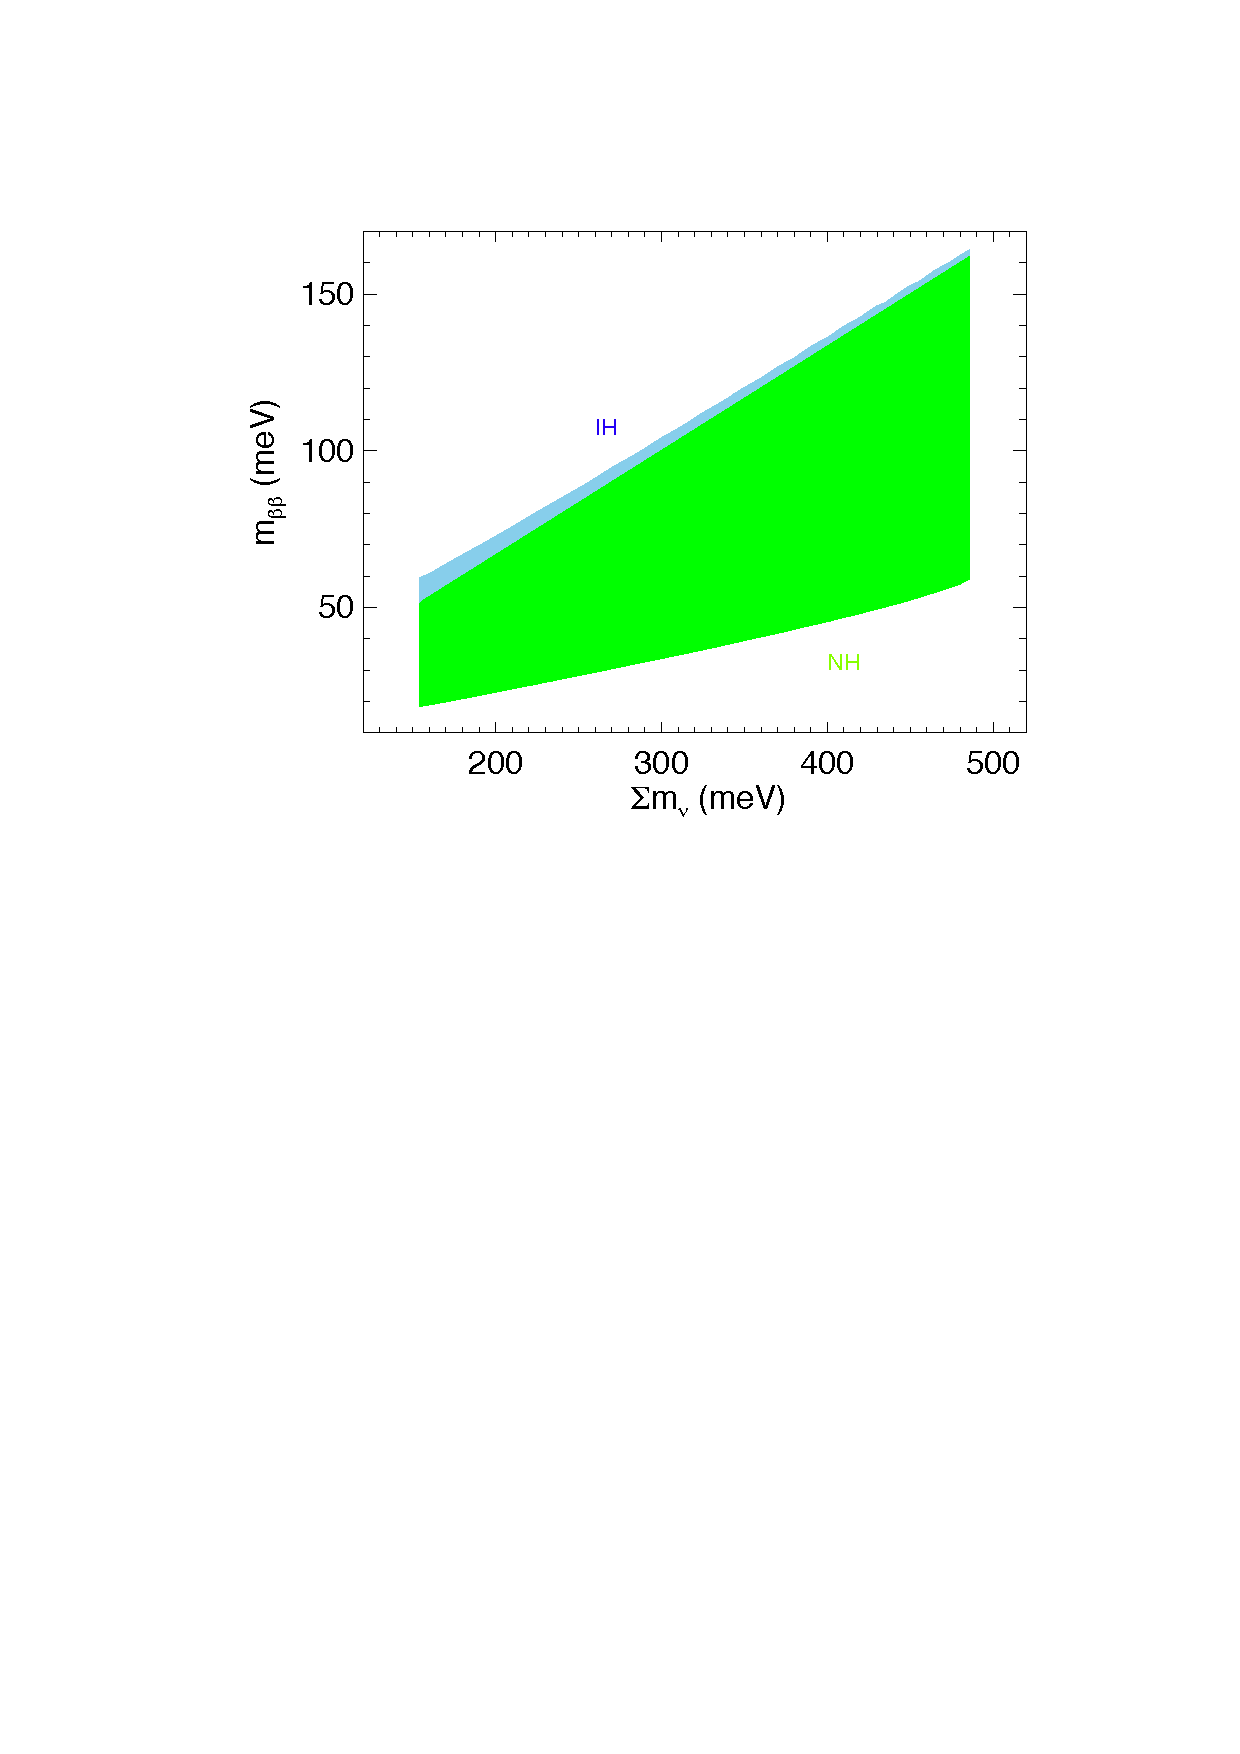
\includegraphics[width=0.65\textwidth]{img/Mbb.pdf}
\caption{The allowed \mbb\ region, as a function of the sum of the neutrino masses, assuming that 
$\sum m_i = 0.32$~eV.} \label{fig.mbb}
\end{figure}
%%%%%%

 Several analysis from recent cosmological results suggest that the sum of the masses of the three neutrinos could be $\sim$ 0.3 eV\footnote{Phys. Rev. Lett. 112, 051303 (2014)}. The PI and collaborators have demonstrated that, in this case, if the neutrino is a Majorana particle, then, $\mbb \sim [20-150]$~ meV \footnote{JCAP 1303 (2013) 043}, as shown in Figure \ref{fig.mbb}. In this scenario, the sensitivity of GERDA is outside the region ``cosmologically relevant region'' (CRR), while both EXO-200 and KamLAND-Zen would have already explored a significant fraction of CRR {\em for the most optimistic NME set} (while they would be outside CRR for the most pessimistic). 
 
 Clearly, the experimental effort to determine if the neutrino is a Majorana particle, far from being completed is, rather, in its infancy. To establish unambiguously that the neutrino is (or not) a Majorana particle, even in this favourable scenario in which the sum of the neutrino masses is relatively high, experiments must be sensitive to $\mbb \sim 20$~meV, {\em even for the most pessimistic NME} set. On the other hand, a xenon experiment probing a $\Tonu >2.6 \times 10^{25}$~yr, has chances of making a discovery.
 
 
%%%%%%%%%%%%%%%%%%%%%%%%%%%%%%%%%%%%%%%%%%%%%%%%%%%%%%%%%%%%
\subsubsection*{The NEXT experiment and its innovative concepts}
\begin{figure}
\centering
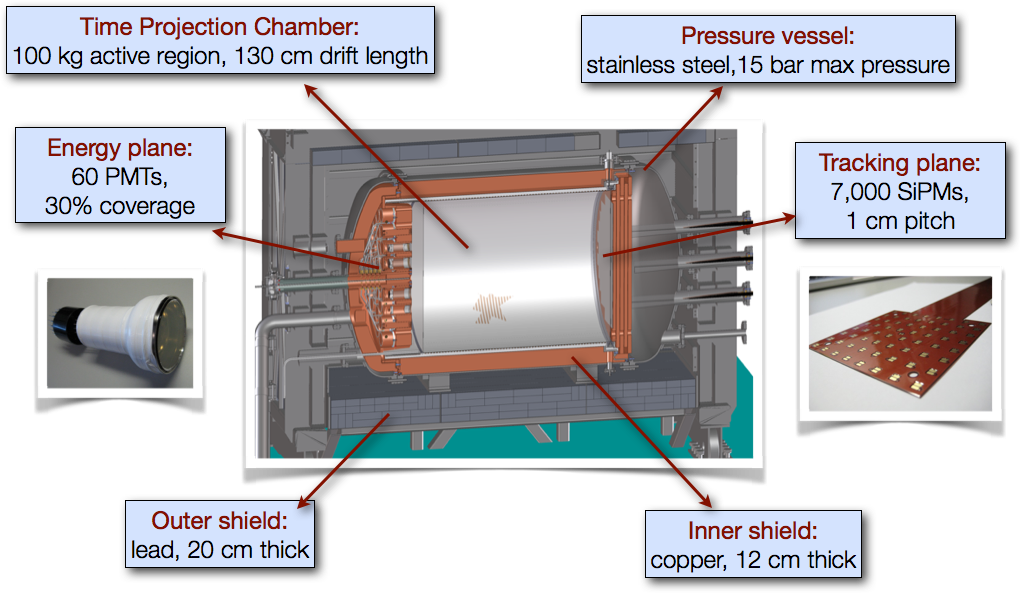
\includegraphics[width=0.9\textwidth]{img/NEXT.png}
\caption{\small A drawing of the NEXT-100 detector showing its main parts.} \label{fig.NEXT100}
\end{figure}

The \emph{Neutrino Experiment with a Xenon TPC} (NEXT)\footnote{\href{http://next.ific.uv.es/}{http://next.ific.uv.es/}} will search for \bbonu\ in \XE\ using  high-pressure xenon gas  time projection chambers (\HPXE). The advantages of the technology are: 
a) {\bf excellent energy resolution}, with an intrinsic limit of about 0.3\% FWHM at \Qbb, close to that of \GE\ detectors; b)
{\bf tracking capabilities} that provide a powerful topological signature to discriminate between signal (two electron tracks with a common vertex) and background (mostly, single electrons); c)
{\bf a fully active and homogeneous detector}, with no dead regions; d) {\bf scalability} of the technique to larger masses; e) the possibility of exciting the barium ion produced in the xenon decay from the fundamental state \TwoS\ to the state \TwoP, using a ``blue'' laser (493.54 nm), and observing the ``red light'' emitted in the transition from \TwoP to \TwoD, thus ``tagging'' the presence of a barium atom in the xenon gas, which cannot be produced by any known background. 

The design of the NEXT chambers is optimised for energy resolution by using proportional electroluminescent (EL) amplification of the ionisation signal. The detection process involves using the prompt scintillation light from the gas as start-of-event time, drifting the ionisation charge to the anode by means of an electric field ($\sim0.3$ kV/cm at 15 bar) where secondary EL scintillation will be produced in the region defined by two highly transparent meshes, between which there is a field of $\sim20$ kV/cm at 15 bar. The detection of EL light provides an energy measurement (in the energy plane, made of PMTs, located behind the cathode) as well as providing tracking through its detection a few mm away from production at the anode plane, via a dense array (1 cm pitch) of 1-mm$^{2}$ SiPMs (the \emph{tracking plane}).

The design of the NEXT-100 detector (Figure \ref{fig.NEXT100}) has been described in a \emph{Technical Design Report}.\footcite{Alvarez:2012haa} NEXT-100 has the structure of a Matryoshka (a russian nesting doll). The outermost layer is a shield made of lead, which attenuates the background from the LSC rock by 6 orders of magnitude (e.g., the \TL\ photons are attenuated from $\sim 10^{12}$~per year to $\sim 10^{6}$~per year). The pressure vessel, built out of steel, can hold 150 kg of xenon at 15 bar. Finally, an inner copper shield, 12 cm thick, constitutes the innermost and more radio-clean layer of the Matryoshka. In addition, all NEXT components have been selected and screened for low background. Of particular importance are the PMTs, whose activity is only 0.4 mBq of \BI\ and 0.3 mBq of \TL\ per unit. Our TDR included a detailed background model. A recent paper has validated these results from measurements in a extensive screening campaign carried out in the past year.\footcite{Alvarez:2012as} Currently, most of the major components entering the NEXT detector have been measured, and those numbers are incorporated in our background model. 

%%%%%%%%%%%%%%%%%%%%%%%%%%%%%%%%%%%%%%%%%%%%%%%%%%%%%%%%%%%%
\subsubsection*{NEXT prototypes}

%%%%%%%%%
%%%%%%%%%
\begin{figure}
\centering
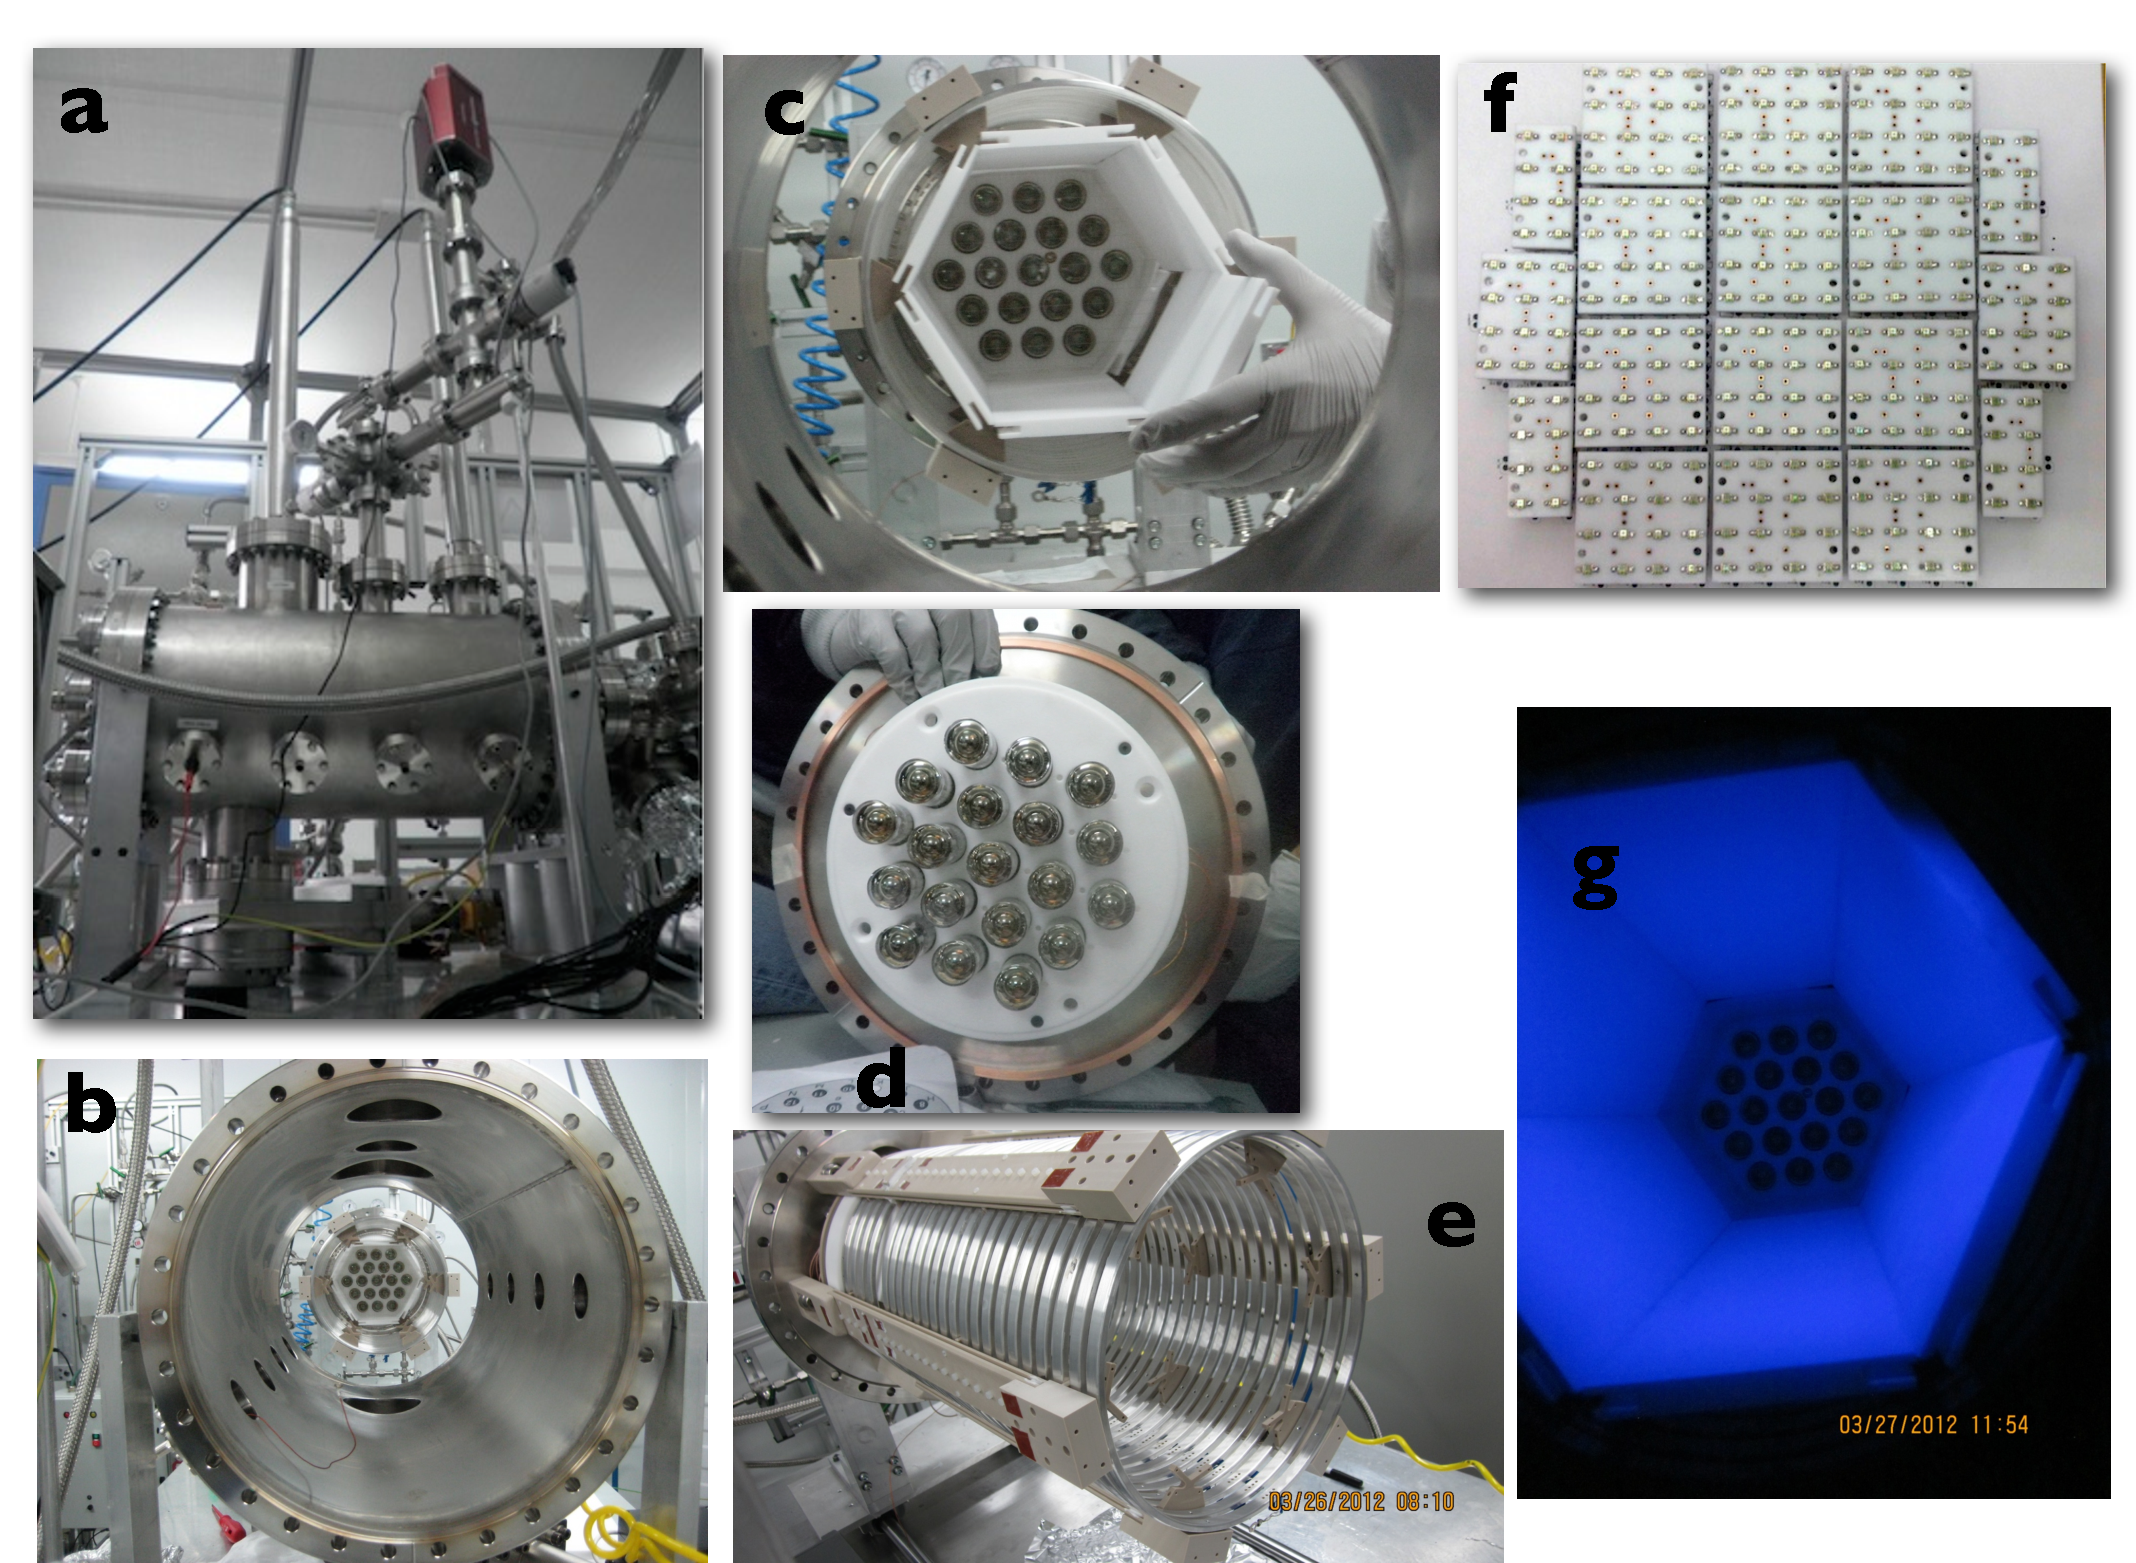
\includegraphics[width=0.7\textwidth]{img/DEMO.pdf}
\caption{\small The NEXT-DEMO prototype. (a) The pressure vessel, showing the HVFT and the mass spectrometer; (b) an expanded view of the detector; (c) Teflon light tube; (d) energy plane, made of pressure resistant Hamamatsu R7378A PMTs; (e) field cage; (f) tracking plane equipped with 300 Hamamatsu MPPCs; (g) Light tube coated with TPB, reflecting UV light in blue.} \label{fig.DEMO}
\end{figure}
%%%%%%%%%%

From 2009 to 2013 the NEXT Collaboration has carried out an intense R\&D program that has culminated in the construction, commissioning and operation of the NEXT-DEMO prototype located at IFIC, and the NEXT-DBDM prototype operating at LBNL. The description of these prototypes and the initial results obtained with them have recently been published\footcite{Alvarez:2012hh, Alvarez:2012nd, Alvarez:2012hu}.

NEXT-DEMO, shown in figure \ref{fig.DEMO}, is as a large-scale prototype of NEXT-100. The pressure vessel has a length of 60 cm and a diameter of 30 cm. The vessel can withstand a pressure of up to 15 bar. The maximum capacity of the detector is 10 kg but in its current configuration (the fiducial volume is an hexagon of 16 cm diameter and 30 cm length) it holds 4 kg at 15 bar. NEXT-DEMO is  equipped with an energy plane made of 19 Hamamatsu R7378A PMTs and a tracking plane made of 300 Hamamatsu MPPCs. 

The detector has been operating successfully for more than one year and has demonstrated: (a) very good operational stability, with no leaks and very few sparks; (b) good energy resolution ; (c) track reconstruction with PMTs and with SiPMs coated with TPB; (d) excellent electron drift lifetime, of the order of 20 ms. In summary, the operation of NEXT-DEMO has been instrumental in the development of the required knowledge to design and build the NEXT detector.

The NEXT-DBDM prototype is a smaller chamber, with only 8 cm drift, but an aspect ratio (ratio diameter to length) similar to the NEXT detector. The device has been used to perform detailed energy resolution studies. NEXT-DBDM achieves a resolution of 1\% FWHM at 660 keV and 15 bar, which extrapolates to 0.5\% at \Qbb.

\subsubsection*{Topological signature}

%%%%%
\begin{figure}
\centering
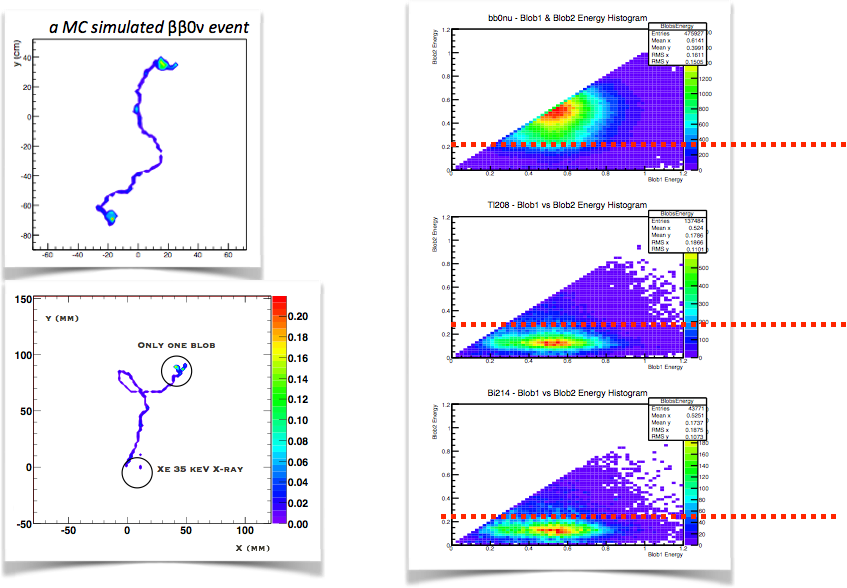
\includegraphics[width=0.9\textwidth]{img/Topology.png}
\caption{\small NEXT has a topological signature, not available in most \bbonu\ detectors. The panel shows the reconstruction of a Monte Carlo signal (left) and background (right) event. The signal has two electrons (two blobs). The background has only one electron (one blob) and the associated emission of a 35 keV X-ray. The color codes energy deposition in the TPC. An scatter plot of the energy of the two blobs shows a clear separation between signal and background regions.}\label{fig.ETRK2}
\end{figure}
%%%%%
	
Double beta decay events leave a distinctive topological signature in HPXe: a continuous track with larger energy depositions (\emph{blobs}) at both ends due to the Bragg-like peaks in the d$E$/d$x$ of the stopping electrons (figure \ref{fig.ETRK2}, topleft). In contrast, background electrons are produced by Compton or photoelectric interactions, and are characterised by a single blob and, often, by a satellite cluster corresponding to the emission of $\sim30$-keV fluorescence x-rays by xenon (figure \ref{fig.ETRK2}, bottonleft).
Reconstruction of this topology using the tracking plane provides a powerful means of background rejection, as can be observed in the figure. In our TDR we chose a conservative cut to separate double--blob from single--blob events which provided a suppression factor of 20 for the background while keeping 80\% of the signal.  

%The NEXT-DEMO prototype has demonstrated that electron tracks can be easily characterised in an HPXe TPC. Na-22 electrons, with an energy of 511 keV, have been used to demonstrate an efficiency of single-blob counting larger than 98\% and a frequency of erroneous double blob counting of less than 0.14\%. This is a robust confirmation of the excellent background rejection capability of the technology. 

\subsubsection*{Energy resolution}

%%%%%%
%\begin{figure}
%\centering
%\includegraphics[width=0.7\textwidth]{imgs2/RES.pdf}
%\caption{Energy resolution measured with NEXT-DBDM prototype at  15 bar. Data points show the measured energy resolution for 662 keV gammas (squares), 30 keV xenon X-rays (triangles) and LED light pulses (circles) as a function of the number of photons detected. The expected resolution including the intrinsic Fano factor, the statistical fluctuations in the number of detected photons and the PMT charge measurement variance. The measured resolution extrapolates to $\sim$0.5\% FWHM at \Qbb.}\label{fig.RES}
%\end{figure}
%%%%%

%%%%%
\begin{figure}
\centering
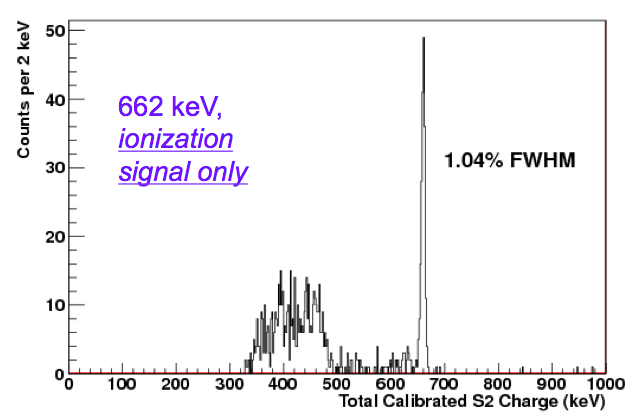
\includegraphics[width=0.6\textwidth]{img/Cs660.png}
\caption{\small The resolution of the photo peak for 662 keV electrons in NEXT-DBDM, at 15 bar is 1\% FWHM (0.5\% FWHM at \Qbb).}\label{fig.ERES}
\end{figure}
%%%%

Figure \ref{fig.ERES} shows the resolution obtained with the NEXT-DBDM apparatus. A resolution of 1\% FWHM with 
662 keV photons, has been measured, which extrapolates to 0.5\% FWHM at \Qbb. This result is not far from the expected limit obtained adding in quadrature the different factors that contribute to the resolution (Fano factor, photoelectron statistics and electronic noise). The resolution measured in NEXT-DEMO extrapolates to 0.7\% FWHM. The difference between both prototypes is due to better photoelectron statistics and aspect ratio in DBDM. The results, are, in any case, better than the target of 1\% FWHM described in the TDR.

The status of the NEXT experiment and the results achieved by the prototypes have been described in a recent
paper \footnote{{\bf Present status and future perspectives of the NEXT experiment},
{\em NEXT Collaboration (J.J. Gomez-Cadenas et al.)}, DOI: 10.1155/2014/907067. 
arXiv:1307.3914 }

%%%%%%%%%%%%%%%%%%%%%%%%%%%%%%%%%%%%%%%%%%%%%%%%%%%%%%%%%%%%

\subsubsection*{The NEW detector}
\label{sec.new}

%%%%%%%%%%
\begin{figure}
\centering
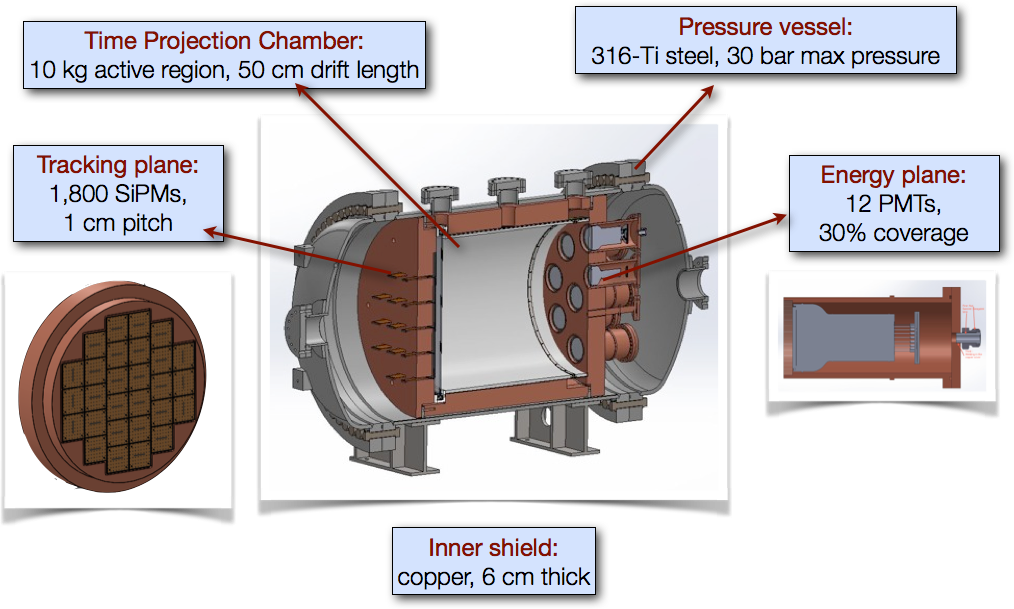
\includegraphics[height=9cm]{img/NEW.png}
\caption{The NEW apparatus.} \label{fig:NEW}
\end{figure} 

The NEW (NEXT-WHITE) apparatus\footnote{The name honours the memory of Professor James White, recently deceased and one of the key scientists of the NEXT Collaboration.}, shown in Figure \ref{fig:NEW} is the first NEXT detector to operate underground. NEW has a triple goal:

\begin{enumerate}
\item {\bf Technology}: it will validate the technological solutions adopted by NEXT-100.
\item {\bf Radiopurity}: it will allow the NEXT collaboration an extra step in the implementation of a radiopure detector.
\item {\bf Physics}: it will demonstrate with measurements of the \BI\ and \TL\ lines, as well as with the measurement of the \bbtnu\ spectrum, the physics capabilities of NEXT-100.
\end{enumerate}

NEW is a scale 1:2 in size (1:8 in mass) of NEXT-100. The energy plane contains 12 radio pure PMTs
of 3 inches diameter, isolated from the gas inside vacuum-tight copper enclosures (we refer to these as PMT cans). The tracking plane technology consists of 30 Kapton Dice Boards (KDB) deploying 1800 SiPMs. The field cage has a diameter of 50 cm and a length of 60 cm. 

The NEXT background model is currently based on a sophisticated Monte Carlo simulation of all expected background sources in each part of the detector. NEW will allow the validation of the background model with the data themselves. Furthermore, it will allow us to identify and correct any possible hot spots, which can only be identified with operating experience.

Furthermore, the calibration of NEW with 
sources of higher energy, will allow a precise study of the evolution of the resolution with the energy. 
In particular it will be plausible to measure the resolution near \Qbb\ using a Thorium source, which provides 2.6 MeV gammas. Last, but not least, we intend to 
reconstruct the spectrum of \bbtnu. Those events are topologically identical to signal events (\bbonu) and can be used to demonstrate with data the power of the topological signature. 

\subsubsection*{Discovery potential of NEXT-100}

The excellent resolution of NEXT (0.5-0.7 \% FWHM) and the combination of low radioactive budget and topological signature (which yields an expected background rate of $5 \times 10^{-4} \ckky$, will allow the NEXT-100 detector to reach a sensitivity on the \bbonu\ period of $\Tonu > 7 \times 10^{25}$~yr for a exposition of 300 kg$\times$yr. This translates in a range for \mbb\ of $[67-187]$~meV. Therefore NEXT-100 will have a substantial chance of making a discovery if the NME is sufficiently high. 

\subsubsection*{Towards a ton-scale high-pressure xenon TPC. BEXT}

%%%%%%
\begin{figure}
\centering
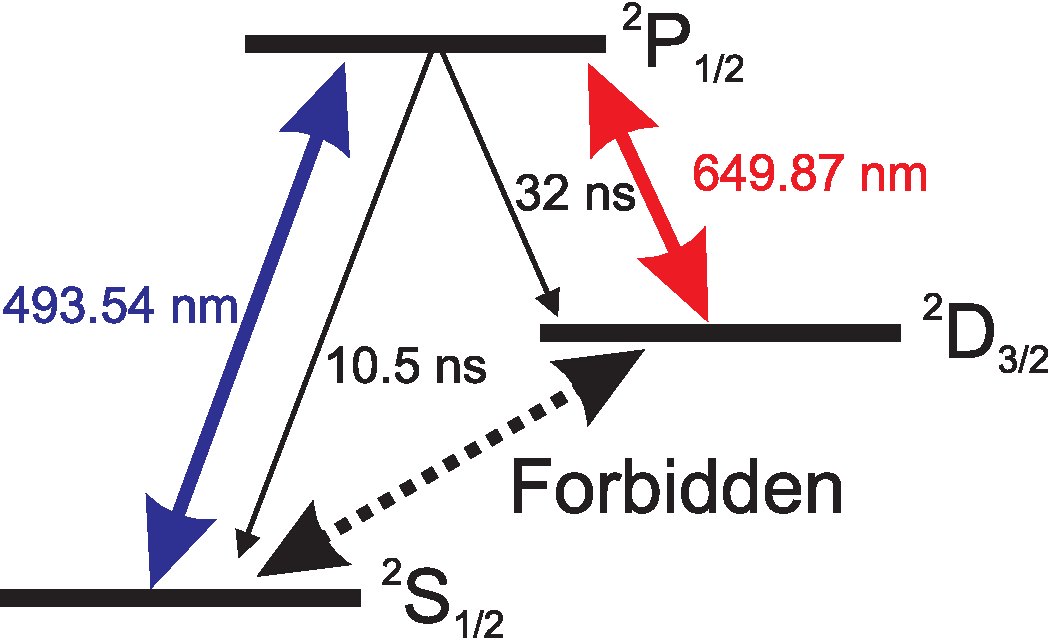
\includegraphics[width=0.65\textwidth]{img/bata.pdf}
\caption{The \BATA\ concept.} \label{fig.BATA}
\end{figure}
%%%%%%

If no discovery is made by the current generation of experiments, the full exploration of the CRR region (corresponding to the inverse hierarchy of neutrino masses) requires detectors of larger mass (at least 1 ton), good resolution and extremely low specific background. The \HPXE\ technology has the potential to provide the most sensitive detector in the ton scale, by scaling the detector to a mass in the range of the ton and adding additional handles to further suppress the background. 

One of the most promising possibilities is to develop the technology to unambiguously tag the barium ion produced in the xenon decay, $Xe \rightarrow Ba^{++} + 2 e$. The conceptual idea to tag $Ba^{+}$ is illustrated in Figure \ref{fig.BATA}. A ``blue'' laser of wavelength 493.54 nm excites (``pumps'') the S state, inducing $S \rightarrow P$~transitions, with a lifetime of $\sim$ 10 ns. About 30 \% of the times the \TwoP\ states decay to the state \TwoD, emitting ``red'' (649.86 nm) fluorescence in a characteristic time of 30 ns. The state \TwoD\ is metastable, but a second laser of suitable wavelength (2051.66 nm) can be used to induce the transition to the ground state (this is known as ``deshelving'').  The whole cycle takes less than 50 ns, and therefore several millions of red fluorescence photons can be emitted by a single ion. 

Of course, the practical application of this beautiful conceptual idea is by no means easy, and in fact, it has been shown to be extremely difficult in liquid xenon by the work of the EXO collaboration. However, it may be feasible in an \HPXE\ detector, where a number of fortunate conditions may occur. Theses conditions are: a) charge reduction of the emitted barium ion, from $Ba^{++}$~to $Ba^{+}$, which can be induced by collisions with xenon atoms, or by the addition of a suitable quencher, such as TEA, as demonstrated by Sinclair et al\footnote{Sinclair.}, b) ``trapping'' of the barium ion ``in situ'' by the surrounding Xe atoms, which result in a very low drift velocity for the ion; c) location of the ion, done by reconstructing the event vertex. 

All the above needs to be demonstrated with a systematic R\&D program, which must also address many other experimental issues such as pressure broadening of the laser, filtering of Rayleigh scattering, etcétera. Most importantly, such an experimental program must be carried out by an interdisciplinary group, combining the experience in laser spectroscopy and atomic physics, with the experience in \HPXE\ instrumentation.

The on-going collaboration between the IFIC (and other groups of NEXT) and the Center for Pulsed Lasers (CLPU) \footnote{http://www.clpu.es}, a national facility dedicated to ultra-intense lasers research and development has made possible to create precisely the interdisciplinary team needed for a successful R\&D program, which can culminate in a ``Barium-tagging Experiment with a Xenon TPC'' (BEXT). We are currently preparing a white paper which describes the theoretical grounds and details the experimental program to be developed\footnote{To be found here}. 

A future detector of 1 ton mass, with a resolution of 0.5 \% FWHM and a background rate in the range of $10^{-6} \ckky$~(thanks to the implementation of barium-tagging) would be able to fully cover the CRR (inverted hierarchy) region in less than 5 years run, assuming a favourable scenario for the NME. Even the most pessimist scenario could be fully explored, however, with a longer run, since the sensitivity to period increases in this case (virtually background free experiment) linearly with exposure. 

Clearly the construction of a ton-scale \HPXE\ detector implementing a full \BATA\ technology is a very challenging enterprise. On the other hand, we believe that the incremental approach devised by the NEXT collaboration will also work in this case. The construction of the NEW detector is progressing without significant problems thanks to the expertise and know-how gained during DEMO phase, and we expect that NEXT-100 will fully benefit from the experience gained with NEW. Similarly, the \BATA\ technology could be ready in a period of 5-7 years, by approaching the problem step by step. 

To conclude, we have shown that the NEXT-100 detector, which we aim to construct, commission and operate during the next few years has a significant potential of making a major discovery. We have also shown that the \HPXE\ technology with \BATA\ included may be the most promising experimental path to find out if the neutrino is its own antiparticle. 
 